%% Forensic Science International: Digital Investigation
%% Elsevier elsarticle class, numbered citation style.
%%
%% Compile with:  latexmk -pdf main.tex
%% Overleaf ships elsarticle, so no local class file is needed there.

\documentclass[preprint,12pt,3p]{elsarticle}

\usepackage{amsmath}
\usepackage{amssymb}
\usepackage{graphicx}
\usepackage{booktabs}
\usepackage{siunitx}
\usepackage[hidelinks]{hyperref}
\usepackage{url}

\sisetup{detect-weight=true, detect-family=true}

\journal{Forensic Science International: Digital Investigation}

\begin{document}

\begin{frontmatter}

\title{What Do AI-Generated Music Detectors Actually Learn?\\
Cross-Generator and Cross-Corpus Evaluation of a\\
MERT-Based Detector with Attention Pooling}

\author[christ]{Laksh}

\affiliation[christ]{organization={Department of Computer Applications,
                                   CHRIST (Deemed to be University)},
                     city={Bengaluru},
                     country={India}}

\begin{abstract}
Generative systems such as Suno and Udio now synthesise complete songs that
listeners struggle to distinguish from human-composed music, and detectors built
to identify them are known to generalise poorly: reported $F_1$ falls from 0.99
in-distribution to 0.629 on an unseen generator. We build a detector on the
frozen MERT music foundation model (\num{94.4}~million parameters) with a
\num{0.62}~million-parameter trainable head that aggregates all thirteen
hidden states by layer attention and pools frames and clips by learned
attention, and we evaluate it under a protocol that separates two failure modes
usually reported as one. On a balanced subset of SONICS (910 songs) the detector
reaches $F_1$ 0.957 with expected calibration error 0.0002. Holding the real
class fixed and withholding an entire generator, transfer is near-complete in
both directions (Suno$\rightarrow$Udio $F_1$ 0.963, Udio$\rightarrow$Suno 0.977;
AUROC $\geq$ 0.9995; $F_1$ degradation $-0.037$ and $-0.023$ against $-0.361$
reported previously). Evaluated on FakeMusicCaps, where five unseen
text-to-music models are paired with a \emph{different} corpus of real music,
the same detector falls to near chance (AUROC 0.598) and labels every real clip
as generated (FPR 1.00, ECE 0.365). The two results reconcile under one
explanation: the detector encodes what its training corpus's real music looks
like rather than what generation leaves behind, so it survives a new generator
but not a new population of real recordings. We further show that naive
evaluation overstates performance---global loudness and dynamic-range
descriptors alone separate the classes at 0.925 AUROC before
normalisation---and that gradient-based temporal explanations are faithful for
real audio but fail entirely for generated audio, indicating that generation
evidence is spectrally distributed rather than temporally localised.
\end{abstract}

\begin{keyword}
AI-generated music detection \sep audio forensics \sep cross-generator
generalisation \sep calibration \sep explainable AI \sep MERT
\end{keyword}

\end{frontmatter}

\section{Introduction}
\label{sec:introduction}

Generative systems such as Suno and Udio synthesise complete songs---vocals,
instrumentation, lyrics and arrangement---that listeners struggle to
distinguish from professionally produced human music. Streaming platforms now
report that a substantial fraction of newly uploaded tracks are machine
generated, which turns detection from an academic question into an operational
requirement for distributors, rights organisations and digital service
providers.

Detection is also a forensic problem, and it inherits the asymmetry of one. A
missed synthetic track costs a platform little. A human artist wrongly flagged
as synthetic may lose income or reputation on the strength of a model's
confidence. Any detector proposed for this setting therefore has to be
characterised not only by how well it separates classes in the conditions it was
trained on, but by how it fails when those conditions change, and by whether the
confidence it reports can be trusted at the operating point where the decision
is actually made.

The literature reports a single headline failure: cross-generator collapse.
Cros Vila et al.~\cite{crosvila2025} benchmark full-song detectors under an
explicit cross-generator protocol and observe $F_1$ falling from 0.99
in-distribution to 0.629 on an unseen generative family. That number is widely
cited as the measure of the generalisation problem. We argue that it conflates
two distinct failures, and that separating them changes what the problem is.

This paper makes four contributions.

\begin{enumerate}
  \item We build a detector on the frozen MERT music foundation
        model~\cite{li2024mert} with a small attention-pooling head, and
        evaluate it under a protocol that varies the generator and the corpus of
        \emph{real} music independently. An ablation shows the head's design is
        not what produces its accuracy: discarding twelve of the thirteen hidden
        states, or replacing attention pooling with a mean, leaves every metric
        unchanged.
  \item We show that these two axes behave completely differently. Withholding
        an entire generator while holding the real class fixed costs almost
        nothing ($F_1$ degradation $-0.037$ and $-0.023$, against $-0.361$
        reported previously). Changing the corpus of real music collapses the
        same detector to near chance (AUROC 0.598) and causes it to label every
        genuine recording as synthetic (FPR 1.00).
  \item We give the explanation that reconciles them: the detector encodes what
        the real music in its training corpus looks like, rather than what
        generation leaves behind. Generalisation to new generators is therefore
        not evidence of generalisation at all.
  \item We report two diagnostics that any future work in this area can apply: a
        shortcut test showing that global loudness and dynamic-range descriptors
        alone separate the classes at 0.925 AUROC before normalisation, and a
        false-positive-rate check on unseen real music that exposes the
        corpus-dependence directly.
\end{enumerate}

We also find that the $F_1$ conventionally reported in this setting can be
actively misleading: on our cross-corpus evaluation the detector's $F_1$ of
0.750 is identical, to four decimal places, to that of a classifier that labels
every input synthetic. Reporting $F_1$ alone would have presented a total
failure as an improvement over the published baseline.

\section{Related work}
\label{sec:related}

\paragraph{Music representation models}
MERT~\cite{li2024mert} is a BERT-style transformer trained with a multi-task
masked-prediction objective guided by a residual vector-quantisation acoustic
teacher and a constant-Q transform musical teacher. It reaches competitive
results across fourteen music information retrieval tasks while remaining
computationally modest, and is released as a reusable feature extractor rather
than a detector, which makes it a natural frozen backbone. Layer-wise analyses
of self-supervised audio models show that depth encodes a transition from
low-level acoustic to higher-level semantic features~\cite{elkheir2025}, which
motivates learned aggregation across layers rather than use of a single layer.

\paragraph{AI-music and synthetic-song detection}
Cros Vila et al.~\cite{crosvila2025} establish the cross-generator protocol and
the $0.99 \rightarrow 0.629$ collapse this work takes as its reference point.
SONICS~\cite{rahman2025sonics} supplies over 97{,}000 songs of real and
end-to-end generated music from Suno and Udio, together with a spectro-temporal
tokeniser that improves long-range modelling. Afchar et al.~\cite{afchar2025icassp}
reframe detection as identifying a neural decoder's fingerprint and report 99.8\%
accuracy while showing candidly that the accuracy is fragile under distribution
shift. FakeMusicCaps~\cite{comanducci2025} extends the problem to attribution
across five text-to-music generators and reports strong closed-set but weak
open-set performance. A frequency-domain analysis~\cite{afchar2025ismir} grounds
detectability in interpretable spectral evidence.

\paragraph{Shortcuts and evaluation validity}
The closest methodological precedent is in singing-voice deepfake detection,
where CtrSVDD~\cite{zang2024ctrsvdd} was constructed specifically to isolate
synthesis artefacts from voice-separation artefacts, and SingFake~\cite{zang2024singfake}
showed that speech-trained models degrade sharply under unseen singers and
codecs. Both warn that pre-processing can confound a classifier. Our shortcut
and bandwidth diagnostics extend that warning to the music setting and make it
measurable.

\paragraph{Explainability for audio detection}
Attention rollout for transformer audio classifiers~\cite{channing2025} frames
transparency as a prerequisite for deployment. Time-domain relevance
attribution~\cite{grinberg2025} identifies which temporal segments drive a
decision, benchmarked against Grad-CAM and SHAP baselines. SHAP has been applied
to spectrogram- and waveform-trained spoofing networks~\cite{yu2024}, and
Mel-spectrogram CNNs with Grad-CAM-style localisation have been used to
highlight fake-indicative regions~\cite{bajwa2025}. These methods target speech
almost exclusively; an early benchmark for explainable machine-generated music
detection~\cite{li2025explainable} notes that explanation fidelity remains an
open metric. Our results bear directly on that: we find temporal attribution
faithful for real audio and unfaithful for generated audio.

\section{Method}
\label{sec:method}

\subsection{Architecture}

The detector is a frozen MERT-v1-95M backbone with a small trainable head.
Audio is resampled to \SI{24}{\kilo\hertz} mono and segmented into fixed clips;
MERT returns thirteen hidden states per clip at \SI{74.8}{\hertz}, each of
dimension 768. The head aggregates these in three stages.

\paragraph{Per-layer normalisation.}
The thirteen states already share a shape, but differ substantially in scale.
Without normalisation the layer-attention softmax tracks magnitude rather than
informativeness, so each state is passed through its own layer normalisation
before weighting.

\paragraph{Layer attention.}
A learned scalar per layer, softmax-normalised, produces a weighted sum over
depth. Learning one global profile rather than a per-example weighting keeps the
weights readable as an explanation: they state which depths the detector relies
on in general.

\paragraph{Temporal and clip pooling.}
Additive attention pools frames within a clip, and a second attention stage
pools clips within a song. The second stage is necessary rather than
decorative. SONICS songs run \SIrange{32}{240}{\second}, MERT was pre-trained on
\SI{5}{\second} clips, and its attention is $O(T^2)$: at \SI{74.8}{\hertz} a
\SI{120}{\second} song is roughly 9000 frames, whose attention matrix alone
exceeds \SI{1.9}{\giga\byte} per layer in half precision. Audio must therefore
be segmented, and without a song-level stage the model emits per-clip decisions
while the task, and the published baselines, are per-song.

The backbone contributes \SI{94.4}{\mega\nothing} frozen parameters and the head
\SI{0.62}{\mega\nothing} trainable ones.

\subsection{Classification heads and calibration}

The primary output is a binary real/synthetic logit; an auxiliary head predicts
the four-way SONICS taxonomy and is down-weighted so it cannot dominate the
objective that is reported. Probabilities are calibrated by temperature scaling
fitted on validation, never on the evaluation set.

Choosing the operating point required care. When validation separates the
classes completely---which it does here---the conventional choice of the
$(1-\alpha)$ quantile of scores on real music places the threshold immediately
against the real class. That threshold is valid on validation and catastrophic
elsewhere: applied to a shifted distribution it labels everything synthetic. We
instead place the threshold at the midpoint of the separating margin, which
scores identically on validation but is maximally distant from both classes and
therefore far more likely to survive a shift. Section~\ref{sec:results}
quantifies the difference: the quantile threshold yields FPR 1.00 on the
cross-corpus evaluation, the midpoint threshold FPR 0.00 on the cross-generator
one.

\subsection{Explanation layer}

Three levels are produced for every explained song.

\textbf{Level 1} reports the learned attention weights over layers, frames and
clips, which the architecture yields at no cost.

\textbf{Level 2} localises evidence in the signal. MERT consumes raw waveform
through a one-dimensional convolutional stack whose output is
$512~\text{channels} \times \text{time}$; no time--frequency map exists anywhere
in the forward graph. Gradient-based attribution taken there localises
\emph{when}, not \emph{at which frequency}, and we report it as such (Level 2a).
For frequency evidence we occlude tiles in the short-time Fourier domain and
resynthesise, which measures what the model does when a band is actually absent
(Level 2b); this is expensive and is applied to an audit subset.

\textbf{Level 3} computes exact Shapley values over the thirteen layers, treating
each hidden state as a player and the logit under a renormalised subset as the
coalition value. With thirteen layers the $2^{13}$ coalitions are affordable
because the frozen backbone runs once and only the small head is re-evaluated.

Levels 1 and 3 answer different questions---what the model weights, versus what
moved a particular decision---and we report their disagreement rather than
averaging it away.

\subsection{Explanation faithfulness}

No explanation is reported without being scored. We mask the regions an
explanation marks important and measure the movement in the logit against
masking randomly chosen regions of the same extent. The quantity reported is the
\emph{gap} against that random baseline, not the raw deletion curve: masking any
audio degrades a detector somewhat, so a steep curve alone establishes nothing.

\section{Evaluation protocol}
\label{sec:protocol}

The protocol is the paper's main methodological contribution, so we state the
rules it enforces and why each exists.

\subsection{Splitting}

Splits are by song, never by clip. A song yields four clips at \SI{5}{\second}; if clips
of one song fall on both sides, the model can recognise the song rather than the
generator. Splits are stratified by the four-way taxonomy so that rare
sub-classes are represented everywhere.

We note a property of SONICS's own published splits that appears not to have
been reported: its \texttt{id} field links a real song to the synthetic tracks
generated from it, and 4{,}349 source identifiers---12.9\% of rows---appear in
more than one official split. A real recording can therefore sit in the test set
while a track generated from its lyrics and style sits in validation. We report
this rather than repairing it, since re-splitting forfeits comparability with
published figures.

\subsection{Removing shortcuts before measuring}

Before any detector is trained we ask whether the classes are separable without
reference to generation at all, by fitting a linear model on eight global
descriptors of the recording---loudness, crest factor, spectral rolloff,
centroid, zero-crossing rate and high-frequency energy share. None of these
describe how audio was produced; a large AUROC means a 94-million-parameter
transformer will find the same shortcut immediately.

The first such test returned \textbf{0.925 AUROC}. Commercial releases are
mastered loud and heavily compressed while generated tracks are not, so loudness
and crest factor alone carried the classification. Peak normalisation reduced
this to 0.840 and root-mean-square normalisation to 0.821; crest factor is
scale-invariant and survives both. Randomising dynamic range---applied to both
classes and to evaluation as well as training, since the aim is to remove a
confound from the task rather than to augment one split---brought the residual
to \textbf{0.714}, and to \textbf{0.737} on the final 910-song corpus. We report
detector performance only against that baseline.

A second diagnostic compares the spectral bandwidth of the two classes. Real
audio fetched from streaming sources at one bitrate and generated audio
distributed at another are trivially separable on codec artefacts. We match the
bitrate distribution of the real class to the generated set and verify that the
median spectral-rolloff ratio falls below a fixed threshold before reporting any
figure.

\subsection{Three evaluation axes}

\paragraph{In-distribution.}
Held-out songs, same generators, same corpus. A sanity number.

\paragraph{Cross-generator, shared corpus.}
SONICS contains both Suno and Udio. Training on one and testing on the other
isolates the generator: corpus, pipeline, processing and real class are all held
fixed. Real songs are divided disjointly between the halves, and both directions
are run because transfer is not symmetric in general.

\paragraph{Cross-corpus.}
FakeMusicCaps pairs five unseen text-to-music generators with real music from
MusicCaps. Here the generator \emph{and} the corpus of real music change
together. We band-limit the real clips to the generated set's sample rate and
verify bandwidth before reporting.

\subsection{Reporting rules}

Every cross-generator result is reported beside the $F_1$ that a classifier
labelling all inputs synthetic would obtain on the same class balance. This is
not a formality: our own cross-corpus $F_1$ of 0.750 matches that baseline to
four decimal places. AUROC and false-positive rate are reported alongside $F_1$
throughout, because $F_1$ alone cannot distinguish a working detector from a
degenerate one.

\section{Results}
\label{sec:results}

\subsection{Setup}

The corpus is a balanced subset of SONICS: 910 songs, 455 per class, real music
fetched from the source identifiers SONICS provides and generated music drawn
from its released archives. Clips are \SI{5}{\second}, four per song. After
decoding, 816 songs remained usable (361 real, 455 synthetic). The shortcut
diagnostic on this corpus reads 0.737 AUROC, below the threshold at which we
regard a detector score as interpretable.

\subsection{In-distribution}

On the held-out split ($n = 122$) the detector reaches $F_1$ 0.957, accuracy
0.951, AUROC 1.000 and expected calibration error $1.54\times10^{-4}$.
Validation $F_1$ reaches 1.000 at the first epoch and remains there, so this
figure is saturated and should be read as a ceiling rather than a measurement of
architectural quality (Section~\ref{sec:limitations}).

\subsection{What the architecture contributes}

The detector's novelty claim rests on the head: learned attention over all
thirteen MERT layers, and learned attention rather than averaging when pooling
frames and clips. Table~\ref{tab:ablation} replaces each of those choices in
turn, retraining from the same seed on the same split.

\begin{table}[t]
\centering
\caption{Pooling and layer ablations ($n = 122$, 55 real). Every variant is
retrained from the same seed. The three left-hand columns are identical to
every digit across the first three rows; the entire spread across all four
architectures is one song.}
\label{tab:ablation}
\begin{tabular}{lSSSS}
\toprule
Variant & {$F_1$} & {AUROC} & {FPR} & {ECE} \\
\midrule
Layer attention + attention pooling (full) & 0.9926 & 1.000 & 0.018 & 0.0041 \\
Mean frame pooling                         & 0.9926 & 1.000 & 0.018 & 0.0082 \\
Last hidden state only                     & 0.9926 & 1.000 & 0.018 & 0.0073 \\
Mean clip$\rightarrow$song pooling         & 1.0000 & 1.000 & 0.000 & 0.0001 \\
\bottomrule
\end{tabular}
\end{table}

The result is negative and we report it as such. Discarding twelve of the
thirteen hidden states changes nothing. Replacing attention over frames with an
unweighted mean changes nothing. Read as counts rather than rates, the first
three rows each classify 121 of 122 songs correctly and each make the same
single false positive out of 55 real songs; the fourth makes none. The full
range of the table is one song, which is not a difference any of these
architectures can be credited with.

Two things follow. The architectural contribution is not measurable on this
corpus, so the case for the design has to rest on the explanations it makes
available---which Section~\ref{sec:discussion} argues is where its value
actually lies---rather than on accuracy. And the one variant that is not
identical is mean clip-to-song pooling, which is nominally the \emph{best} row.
We draw no conclusion from that either: a single song separates it from the
rest, and the run is one seed.

What the table cannot do is discriminate, because validation $F_1$ reaches 1.000
at the first epoch for every variant (Section~\ref{sec:limitations}). A corpus
that separates this easily cannot rank heads. The honest reading is that this
experiment is not yet informative, not that the choices are equivalent in
general.

\subsection{Robustness}

Table~\ref{tab:robustness} reports degradation under six held-out perturbations,
none seen during training.

\begin{table}[t]
\centering
\caption{Robustness to held-out degradations ($n = 122$). AUROC is largely
preserved while $F_1$ falls, indicating that discrimination survives but the
operating point does not.}
\label{tab:robustness}
\begin{tabular}{llSS S}
\toprule
Condition & Family & {$F_1$} & {AUROC} & {$\Delta F_1$} \\
\midrule
Clean            & ---    & 0.957 & 1.000 & 0.000 \\
Time stretch     & time   & 0.912 & 1.000 & -0.046 \\
Reverb           & room   & 0.788 & 1.000 & -0.169 \\
Low-pass \SI{4}{\kilo\hertz} & filter & 0.775 & 0.989 & -0.183 \\
MP3 \SI{32}{\kilo\bit\per\second} & codec & 0.766 & 0.944 & -0.191 \\
Pitch shift      & pitch  & 0.724 & 0.999 & -0.233 \\
Additive noise   & noise  & 0.709 & 0.904 & -0.248 \\
\bottomrule
\end{tabular}
\end{table}

The pattern matters more than the magnitudes. Under four of six conditions AUROC
remains at or above 0.989 while $F_1$ falls by up to 0.233. The detector's
ability to rank synthetic above real audio is robust; the threshold at which
that ranking becomes a decision is not. A study reporting $F_1$ alone would
describe this as a robustness failure, when it is a calibration failure.

\begin{figure}[t]
\centering
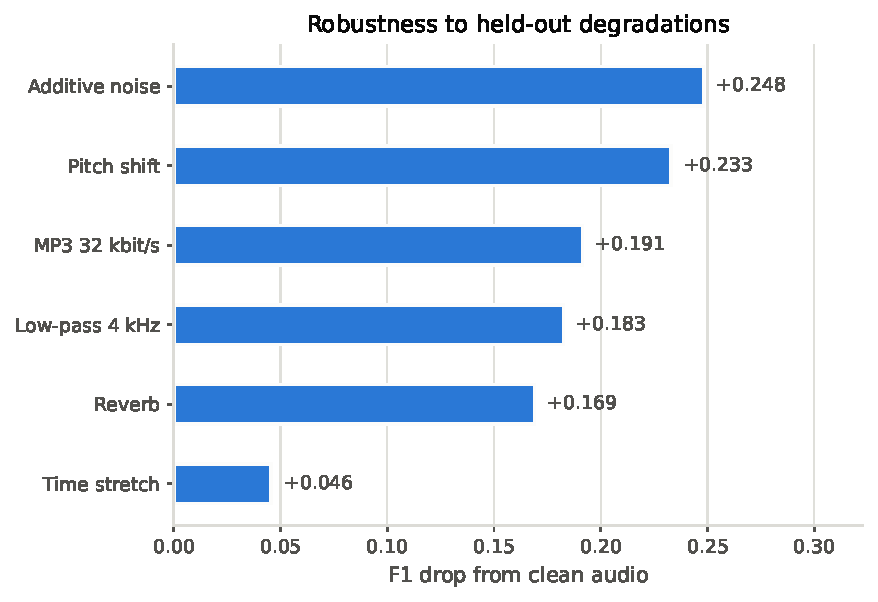
\includegraphics[width=\textwidth]{figures/fig_robustness.pdf}
\caption{$F_1$ loss under each held-out degradation, grouped by perturbation
family. No condition was seen during training. The ordering is not the one a
codec-artefact account of detection would predict: pitch shift and additive
noise cost more than \SI{32}{\kilo\bit\per\second} MP3.}
\label{fig:robustness}
\end{figure}

\subsection{Cross-generator with a shared corpus}

Table~\ref{tab:gensplit} reports both Suno/Udio directions. Each is trained on
one generator and tested on the other, with real songs divided disjointly and
both classes balanced in each half.

\begin{table}[t]
\centering
\caption{Cross-generator transfer within SONICS ($n = 362$ per direction). The
all-positive baseline is 0.667; both results are well clear of it.}
\label{tab:gensplit}
\begin{tabular}{lSSSSS}
\toprule
Direction & {In-dist. $F_1$} & {Cross $F_1$} & {Cross AUROC} & {FPR} & {ECE} \\
\midrule
Suno $\rightarrow$ Udio & 1.000 & 0.963 & 0.9995 & 0.000 & 0.031 \\
Udio $\rightarrow$ Suno & 1.000 & 0.977 & 1.0000 & 0.000 & 0.022 \\
\bottomrule
\end{tabular}
\end{table}

Degradation is $-0.037$ and $-0.023$ in $F_1$, against the $-0.361$ reported by
Cros Vila et al. False-positive rate is zero in both directions and calibration
error remains near 0.03. Withholding an entire generative family, with the real
class held fixed, costs the detector almost nothing.

\subsection{Cross-corpus}

Evaluated on FakeMusicCaps---five unseen text-to-music generators (AudioLDM2,
MusicGen, MusicLDM, Mustango, StableAudioOpen; 75 clips each) against 250
MusicCaps recordings---the same detector reaches AUROC 0.598, marginally above
chance, with ECE 0.365 and \textbf{FPR 1.00}. Per generator, AUROC ranges from
0.438 (AudioLDM2, below chance) through 0.512, 0.618 and 0.654 to 0.770
(Mustango).

The reported $F_1$ is 0.750. A classifier labelling every input synthetic scores
0.750 on this class balance. The detector has labelled every clip synthetic, and
the figure is the class ratio, not a result. Had we reported $F_1$ against the
published 0.629 baseline we would have claimed a $+0.121$ improvement for a
total failure.

\subsection{The two results together}

Figure~\ref{fig:transfer} places them side by side. Discrimination and
recognition-of-real-music move together and identify the mechanism: FPR 1.00
means every genuine MusicCaps recording was called synthetic. The detector did
not fail to recognise new generators; it failed to recognise new real music.

\begin{figure}[t]
\centering
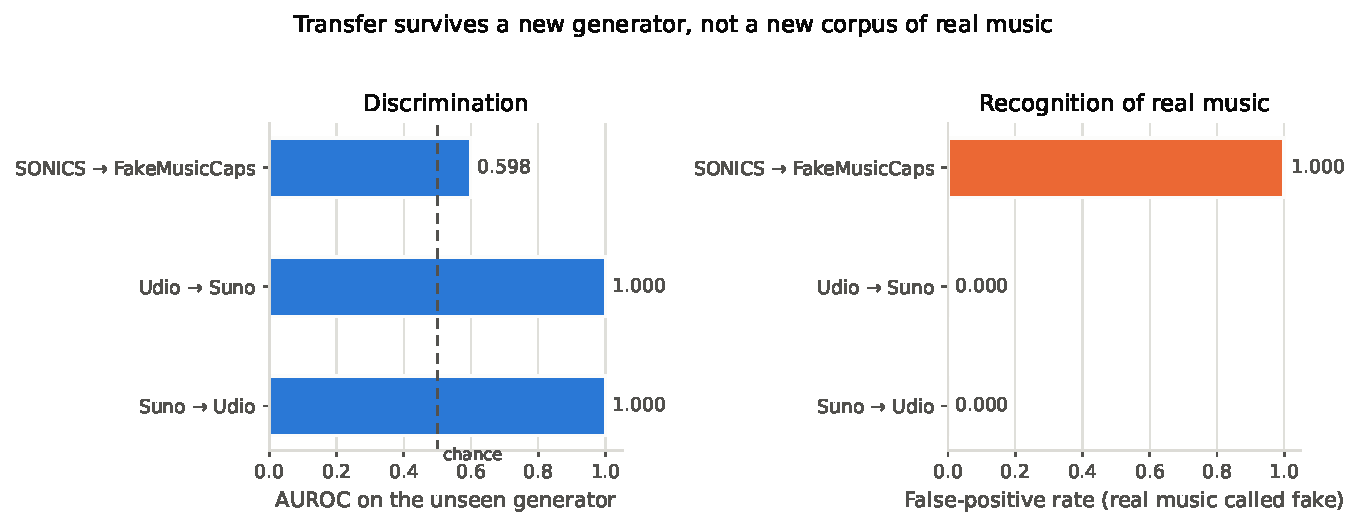
\includegraphics[width=\textwidth]{figures/fig_transfer.pdf}
\caption{Transfer survives a new generator but not a new corpus of real music.
Left: AUROC on the unseen generator. Right: the fraction of genuine recordings
labelled synthetic. With the real class held fixed (Suno/Udio) AUROC is $\geq
0.9995$ and FPR is zero; when the corpus of real music also changes
(FakeMusicCaps) AUROC falls to 0.598 and every real clip is misclassified.}
\label{fig:transfer}
\end{figure}

\subsection{Explanation faithfulness}

Across twelve explained songs, balanced by class, every explanation of a real
recording beat its random baseline (6/6, mean gap $-2.97$) and no explanation of
a generated recording did (0/6, mean gap $+1.31$). For synthetic audio, masking
the regions the explanation marks as important moves the logit \emph{less} than
masking at random. Figure~\ref{fig:faithfulness} shows the deletion curve for
one real recording, where the explanation-ordered curve stays below the random
one across the whole sweep.

\begin{figure}[t]
\centering
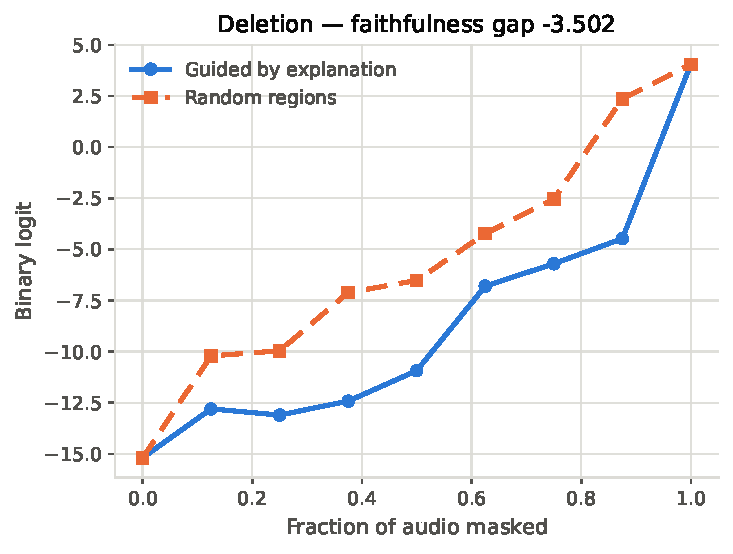
\includegraphics[width=0.78\textwidth]{figures/fig_faithfulness.pdf}
\caption{Deletion curve for a real recording (\texttt{real\_27619},
faithfulness gap $-3.50$). Audio is masked in order of attributed relevance
(solid) or at random (dashed) and the binary logit is re-measured. The
explanation is faithful when its curve sits below the random one, as it does
here across the whole sweep. Every real recording in the audit behaves this way;
no generated one does.}
\label{fig:faithfulness}
\end{figure}

Temporal attribution is therefore inadequate for exactly the class the
application cares about. The evidence a detector uses for ``synthetic'' is not
localised in time, which is consistent with frequency-domain accounts of
AI-music artefacts~\cite{afchar2025ismir} and is a direct argument for
frequency-resolved explanation over Grad-CAM-style temporal methods.

Layer attention converged to a near-uniform profile: weights run 0.073--0.080
about a uniform $1/13 = 0.077$, a spread of 1.09$\times$ between the largest and
smallest. Shapley attribution over the same thirteen layers runs 0.003--0.172, a
spread of 49$\times$, and its coefficient of variation is 20 times the
attention profile's (0.591 against 0.029)
(Figure~\ref{fig:layers}). Worse than uninformative, the two \emph{disagree}:
rank agreement between the attention profile and the Shapley attribution is
negative for every audited song, and strongly so for real recordings (mean
$-0.69$, against $-0.20$ for generated ones; overall $-0.45$). The layers the
model's own gate weights most highly are not the layers whose removal moves the
logit. Reporting Level~1 alone---the explanation the architecture supplies for
free, and the one most readily quoted---would have produced a confident
explanation that the model's behaviour contradicts.

\begin{figure}[t]
\centering
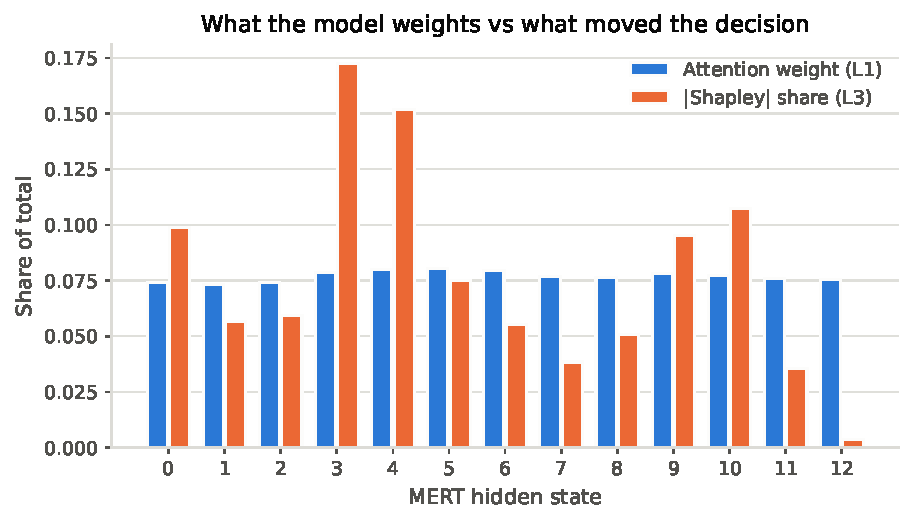
\includegraphics[width=\textwidth]{figures/fig_layers.pdf}
\caption{What the model says it weights against what actually moved the
decision, paired per MERT hidden state. Both quantities are normalised to sum to
one so that a single axis is meaningful. The attention weights (L1) are flat:
0.073--0.080 against a uniform $1/13 = 0.077$, a spread of 1.09$\times$. The
Shapley shares (L3) span 0.003--0.172, a spread of 49$\times$, and concentrate
in the middle of the stack (layers 3--4). The last hidden state, the one a
conventional last-layer probe would use, carries the smallest share of all.}
\label{fig:layers}
\end{figure}

\section{Discussion}
\label{sec:discussion}

\subsection{What the detector learned}

The two cross-generator results are not in tension once the variable that
actually changed is identified. Withholding Suno or Udio changes which
generative process produced the synthetic class; the real class, its corpus, its
provenance and its processing chain all stay fixed, and the detector transfers
almost perfectly. Moving to FakeMusicCaps changes the generative processes
\emph{and} replaces the real class with recordings from a different corpus, and
the detector collapses---specifically, by calling every genuine recording
synthetic.

A detector that had learned the artefacts of generation would degrade on unseen
generators and remain calm on unseen real music. Ours does the opposite. The
most economical reading is that it has learned a model of what real music looks
like in its training corpus, and treats departures from that model as evidence
of synthesis. Under that reading a new generator is simply another departure and
is handled correctly, while genuine music from an unfamiliar corpus is also a
departure and is handled catastrophically.

This has a practical consequence for deployment. A detector validated on
cross-generator splits alone can appear robust and still be unusable, because
the population of real music it will meet in production is never the population
it was trained on. The failure it will exhibit is the expensive one: false
accusation.

\subsection{Why $F_1$ is the wrong headline}

Our cross-corpus $F_1$ of 0.750 exceeds the published cross-generator baseline of
0.629, and means nothing---it is exactly the score of a classifier that labels
everything synthetic. The metric is not defective; it is being asked to do
something it cannot, which is to distinguish a detector from a constant
function when classes are unbalanced.

Two cheap conventions prevent this. Report the all-positive baseline beside every
$F_1$, and report false-positive rate alongside it. Either would have caught our
degenerate result immediately. We would encourage their adoption as a norm in
this literature, where class balance varies widely between evaluation sets and
the cost of a false positive is the main reason the work is being done.

\subsection{Calibration as a first-class result}

The robustness table shows AUROC holding above 0.989 under four of six
degradations while $F_1$ falls by up to 0.233, and the cross-corpus evaluation
shows calibration error rising from $1.5\times10^{-4}$ to 0.365. In both cases
the ranking survives and the decision rule does not.

The mechanism is visible in threshold selection. Where validation separates the
classes perfectly, the usual false-positive-budget threshold lands against the
real class and any distribution shift sweeps the entire real population across
it. Placing the threshold at the midpoint of the separating margin is a one-line
change that moved false-positive rate from 1.00 to 0.00 in our cross-generator
evaluation. Detectors intended for forensic use should report the threshold rule
as part of the method, not as an implementation detail.

\subsection{Explanation, and what it is evidence of}

The faithfulness asymmetry---every explanation of real audio beating its random
baseline, none of generated audio doing so---is a negative result about the
method, not about the model. It says that whatever the detector uses to identify
synthesis is not concentrated in time, and therefore that temporal attribution,
which dominates the audio-explainability literature, cannot surface it.

That is consistent with the frequency-domain characterisation of AI-music
artefacts~\cite{afchar2025ismir}, and it is why we separated the frequency claim
from the temporal one in Section~\ref{sec:method} rather than presenting a
single Grad-CAM-style saliency map over a spectrogram the model never sees.

The layer-level comparison carries a second warning. An attention-pooling
architecture hands the analyst a ready-made explanation---the softmax over
layers---and it is tempting to report it, because it costs nothing and looks
like an answer. In our model it is flat to within 1.09$\times$ and its ordering
is negatively rank-correlated with the exact Shapley attribution over the same
layers in every audited song. The attention weights are not a weak version of
the Shapley values; they point the other way. Architectural attention is
evidence about the architecture, not about the decision, and papers that report
it as an explanation should be read accordingly. This is the concrete payoff of
running Levels~1 and~3 as a contrast rather than as two independent views: the
disagreement is the finding.

\section{Limitations}
\label{sec:limitations}

\paragraph{The in-distribution figure is saturated}
Validation $F_1$ reaches 1.000 at the first epoch and does not move. The
in-distribution result is therefore a ceiling, and the collapses we report are
measured from it. It should not be read as evidence that the architecture is
well matched to the task.

\paragraph{Scale}
The corpus is 910 songs against SONICS's 97{,}164. The real class was fetched
from source identifiers at roughly 85\% coverage, with losses concentrated in
removed, private and region-restricted recordings, so it is not a random sample.
Splits were regenerated after subsampling, so the in-distribution figure is not
directly comparable to SONICS's published results.

\paragraph{Suno and Udio are a close pair}
Both are commercial end-to-end song generators. Near-complete transfer between
them is weaker evidence of generator-independence than transfer between
architecturally distinct families would be, and should not be read as
generalisation to arbitrary generators.

\paragraph{Corpus and generator are confounded in the cross-corpus arm}
FakeMusicCaps changes the corpus, sample rate and clip length together with the
generator. We band-limit and verify bandwidth before reporting, and the FPR of
1.00 on real music localises the failure to the real class specifically, but
isolating the corpus effect cleanly would require a shared real corpus across
both generator families. We regard this as the most important piece of future
work.

\paragraph{The explanation audit is small}
Twelve songs, balanced by class. The separation is complete (6/6 against 0/6),
but the sample is small enough that the effect size, not merely its direction,
needs confirmation at scale.

\paragraph{The ablations cannot rank the architecture}
Every variant reaches validation $F_1$ 1.000 at the first epoch, and the four
differ by a single test song. The table establishes that the pooling and
layer-aggregation choices are not what produces the reported accuracy on this
corpus; it cannot establish that they are equivalent in general, and a harder
corpus may separate them.

\paragraph{Single seed}
Results are from one training run per configuration, including every ablation
variant. Variance across seeds is unmeasured, and with a spread of one song it
would very likely dominate the differences reported in
Table~\ref{tab:ablation}.

\section{Conclusion}
\label{sec:conclusion}

We evaluated a MERT-based AI-music detector under a protocol that varies the
generator and the corpus of real music independently, and found that these two
axes behave completely differently. Withholding an entire generator while
holding the real class fixed costs almost nothing: $F_1$ degrades by 0.037 and
0.023 across the two Suno/Udio directions, against 0.361 reported previously.
Replacing the corpus of real music collapses the same detector to near chance
and causes it to label every genuine recording as synthetic.

The reconciling explanation is that the detector encodes what real music looks
like in its training corpus rather than what generation leaves behind. Strong
cross-generator numbers are therefore not evidence that a detector has learned
to recognise synthesis, and a detector validated on cross-generator splits alone
may fail in deployment in the most costly direction available to it.

We also found that the conventional headline metric conceals this. Our
cross-corpus $F_1$ of 0.750 exceeds the published baseline of 0.629 and is
identical to the score of a classifier that labels every input synthetic.
Reporting the all-positive baseline and the false-positive rate alongside $F_1$
would have made the failure visible at a glance, and we recommend both as
routine practice.

Finally, the explanation layer produced two negative results worth carrying
forward. Gradient-based temporal explanation proved faithful for real audio and
unfaithful for generated audio, indicating that the evidence for synthesis is
not localised in time and that frequency-resolved explanation is the appropriate
tool. And the model's own layer-attention weights---the explanation an
attention-pooling architecture supplies for free---are flat, and their ordering
is negatively rank-correlated with exact Shapley attribution over the same
layers in every song we audited. Architectural attention should be reported as a
property of the architecture, not as an account of the decision.

The immediate next step is an evaluation in which two architecturally distinct
generator families are paired with a \emph{shared} corpus of real music, which
would separate the corpus effect from the generator effect that this work shows
are conflated in current practice.


\section*{Data and code availability}
Code, evaluation protocol and diagnostics are available at\\
\url{https://github.com/Laksh-D25/explainable-aimd}.

\bibliographystyle{elsarticle-num}
\bibliography{references}

\end{document}
